\item A cyclist rides along the circumference of a circular horizontal plane of radius \(R\), the friction coefficient being dependent only on distance \(r\) from the centre \(O\) of the plane as \( k = k_0 (1 - r/R) \), where \( k_0 \) is a constant. Find the radius of the circle with the centre at the point along which the cyclist can ride with the maximum velocity. What is this velocity?
    \begin{center}
        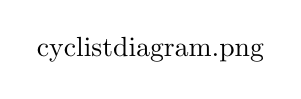
\begin{tikzpicture}
            \node at (0,0) {{cyclistdiagram.png}}; % Assume the diagram is saved as cyclist_diagram.png
        \end{tikzpicture}
    \end{center}

\begin{solution}
    \begin{center}
        \begin{tikzpicture}
            \pic at (0, 0) {frame=3cm};
        \end{tikzpicture}
    \end{center}
    
    \begin{align*}
        \intertext{According to the question, the cyclist moves along the circular path and the centripetal force is provided by the frictional force. Thus from the equation}
        F_n &= mw_n\\
        fr &= \dfrac{mv^2}{r} \quad \text{or} \quad kmg = \dfrac{mv^2}{r}\\
        k_0 \left( 1 - \dfrac{r}{R} \right) g &= \dfrac{v^2}{r} \quad \text{or} \quad v^2 = k_0 \left( r - \dfrac{r^2}{R} \right) g \tag{1}\\
        \intertext{For $v_{\text{max}}$ we should have}
        \dfrac{d}{dr} \left( r - \dfrac{r^2}{R} \right) &= 0\\
        1 - \dfrac{2r}{R} &= 0, \quad \text{so} \quad r = \dfrac{R}{2}\\
        \text{Hence,} \quad v_{\text{max}} &= \dfrac{1}{2} \sqrt{k_0 gR}
    \end{align*}
\end{solution}
